\documentclass[twocolumn, a4paper, 10pt]{article}

% ---- Packages (load before fonts to avoid conflicts) ----
\usepackage{cite}
\usepackage{amsmath,amsfonts}
\usepackage{graphicx}
\usepackage{textcomp}
\usepackage{xcolor}
\usepackage{booktabs}

% ---- Fonts: Times New Roman ----
% newtxmath provides amssymb symbols, so do not load amssymb separately
\usepackage{newtxtext,newtxmath}
\usepackage{geometry}
\usepackage[colorlinks=true, urlcolor=magenta, citecolor=blue, linkcolor=blue]{hyperref}

\geometry{left=1.8cm, right=1.8cm, top=2cm, bottom=2cm}
\graphicspath{{./results/}}

% ---- Section format: Arabic numerals, bold, left-aligned ----
\usepackage{titlesec}
\titleformat{\section}
  {\normalfont\large\bfseries\raggedright}{\thesection}{1em}{}
\titleformat{\subsection}
  {\normalfont\normalsize\bfseries\raggedright}{\thesubsection}{1em}{}
\titleformat{\subsubsection}
  {\normalfont\normalsize\bfseries\raggedright}{\thesubsubsection}{1em}{}

% ---- Abstract: centered title ----
\renewenvironment{abstract}{%
  \begin{center}\normalfont\large\bfseries Abstract\end{center}%
  \itshape\small%
}{}

\begin{document}

\title{\textbf{Image denoising based on self-supervised Neighbor2Neighbor learning}}
\author{Zhang Chengxi}
\date{}
\maketitle

\begin{abstract}
Both supervised denoising methods and the Noise2Noise approach require multiple observations of the same scene---either clean targets or independent noisy pairs. In many practical scenarios, only a single noisy image is available. In this work, we implement a self-supervised denoising model based on the Neighbor2Neighbor (N2N) algorithm. By employing a neighbor sub-sampling strategy with a U-Net backbone, we demonstrate that a network can learn to denoise using only individual noisy images, without any clean targets or paired data. We evaluate the N2N model on the DIV2K dataset with Gaussian noise. Experimental results show that the N2N model achieves reasonable denoising performance, albeit with a modest gap compared to paired methods (Noise2Noise) and supervised approaches, confirming its viability in the most data-constrained scenarios.
\end{abstract}

\section{Introduction}

Image denoising is a fundamental problem in computer vision, aiming to recover a clean image $x$ from a noisy observation $y = x + n$. In previous experiments, we have explored:

(1) \textbf{Exp7}: Supervised U-Net denoising, requiring paired noisy-clean data.

(2) \textbf{Exp8}: Noise2Noise, requiring two independent noisy observations of each scene.

However, in many real-world applications such as medical imaging, satellite imagery, or microscopy, obtaining even two noisy observations of the same scene can be impractical. The Neighbor2Neighbor (N2N) framework addresses this by training a denoiser using only single noisy images. This represents the most relaxed data requirement in our experiment series: from clean targets (exp7) $\to$ noisy pairs (exp8) $\to$ \textbf{single noisy images (exp9)}.

\section{Related work}

Neighbor2Neighbor (Huang et al. \cite{b1}) builds upon the self-supervised denoising principle but eliminates the need for paired data entirely. The key insight is that by generating a pseudo-pair of sub-sampled noisy images from a single noisy image through a neighbor downsampler, one can approximate the Noise2Noise framework. Compared to blind-spot networks like Noise2Void \cite{b2} or Noise2Self \cite{b3}, N2N does not require masking and maintains full spatial correlation, which often yields superior performance.

\section{Methodology}

\subsection{Neighbor2Neighbor principle}

Given a single noisy image $y = x + n$ where the noise $n$ is pixel-wise independent and zero-mean, Neighbor2Neighbor generates a pseudo-pair of noisy observations from $y$ itself. The training procedure is as follows:

(1) \textbf{Sub-sampling}: For each $2 \times 2$ cell in the image, we randomly assign two adjacent pixels (either horizontally or vertically) to two sub-images, $y_1$ and $y_2$. This generates two sub-images of size $H/2 \times W/2$ that represent highly similar structural content but have independent noise realizations.

(2) \textbf{Reconstruction loss}: The network predicts the denoised version of $y_1$ and uses $y_2$ as the target:
\begin{equation}
    \mathcal{L}_{rec} = \|f_\theta(y_1) - y_2\|^2
\end{equation}

(3) \textbf{Regularization loss}: A regularization term $\mathcal{L}_{reg}$ is introduced to prevent trivial solutions, penalizing the difference between the predictions $f_\theta(y_1) - f_\theta(y_2)$ based on the expected difference from the full image prediction $f_\theta(y)$:
\begin{equation}
    \mathcal{L}_{reg} = \lambda \|(f_\theta(y_1) - f_\theta(y_2)) - (\tilde{y}_1 - \tilde{y}_2)\|^2
\end{equation}
where $\tilde{y}_1, \tilde{y}_2$ are sub-sampled from the denoised full image $f_\theta(y)$. The total loss is $\mathcal{L}_{rec} + 2.0 \cdot \mathcal{L}_{reg}$.


\subsection{Network architecture}

For the generator structure, we use the same U-Net encoder-decoder architecture as exp7 and exp8, ensuring a fair comparison across methods. The core innovation of our implementation lies in the downsampling strategy, which constructs two sub-images from a single input to evaluate the reconstruction loss against. Fig.~\ref{fig:n2n_framework} illustrates the overall framework, and Fig.~\ref{fig:unet} shows the U-Net generator architecture.

\begin{figure}[htbp]
    \centerline{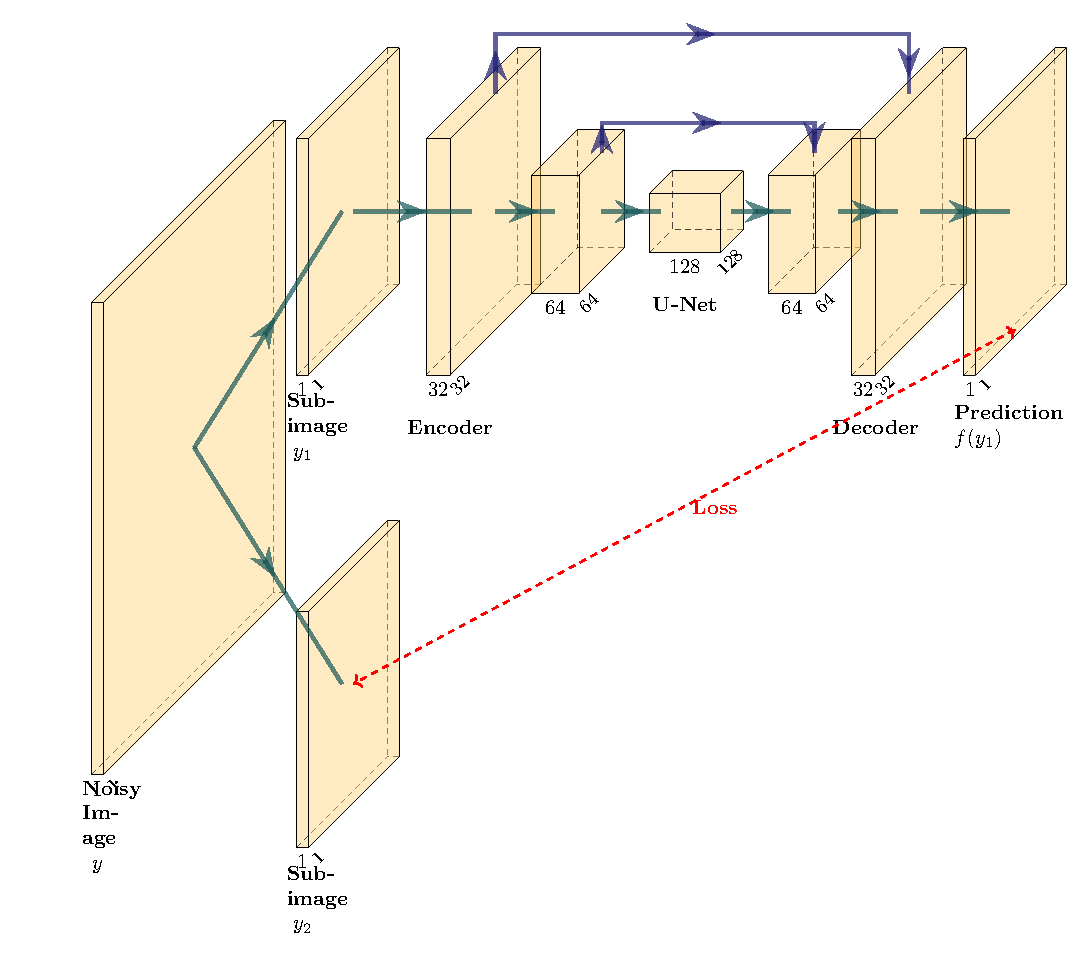
\includegraphics[width=0.48\textwidth]{n2n_framework.pdf}}
    \caption{Neighbor2Neighbor framework: downsampling strategy and loss structure.}
    \label{fig:n2n_framework}
\end{figure}

\begin{figure}[htbp]
    \centerline{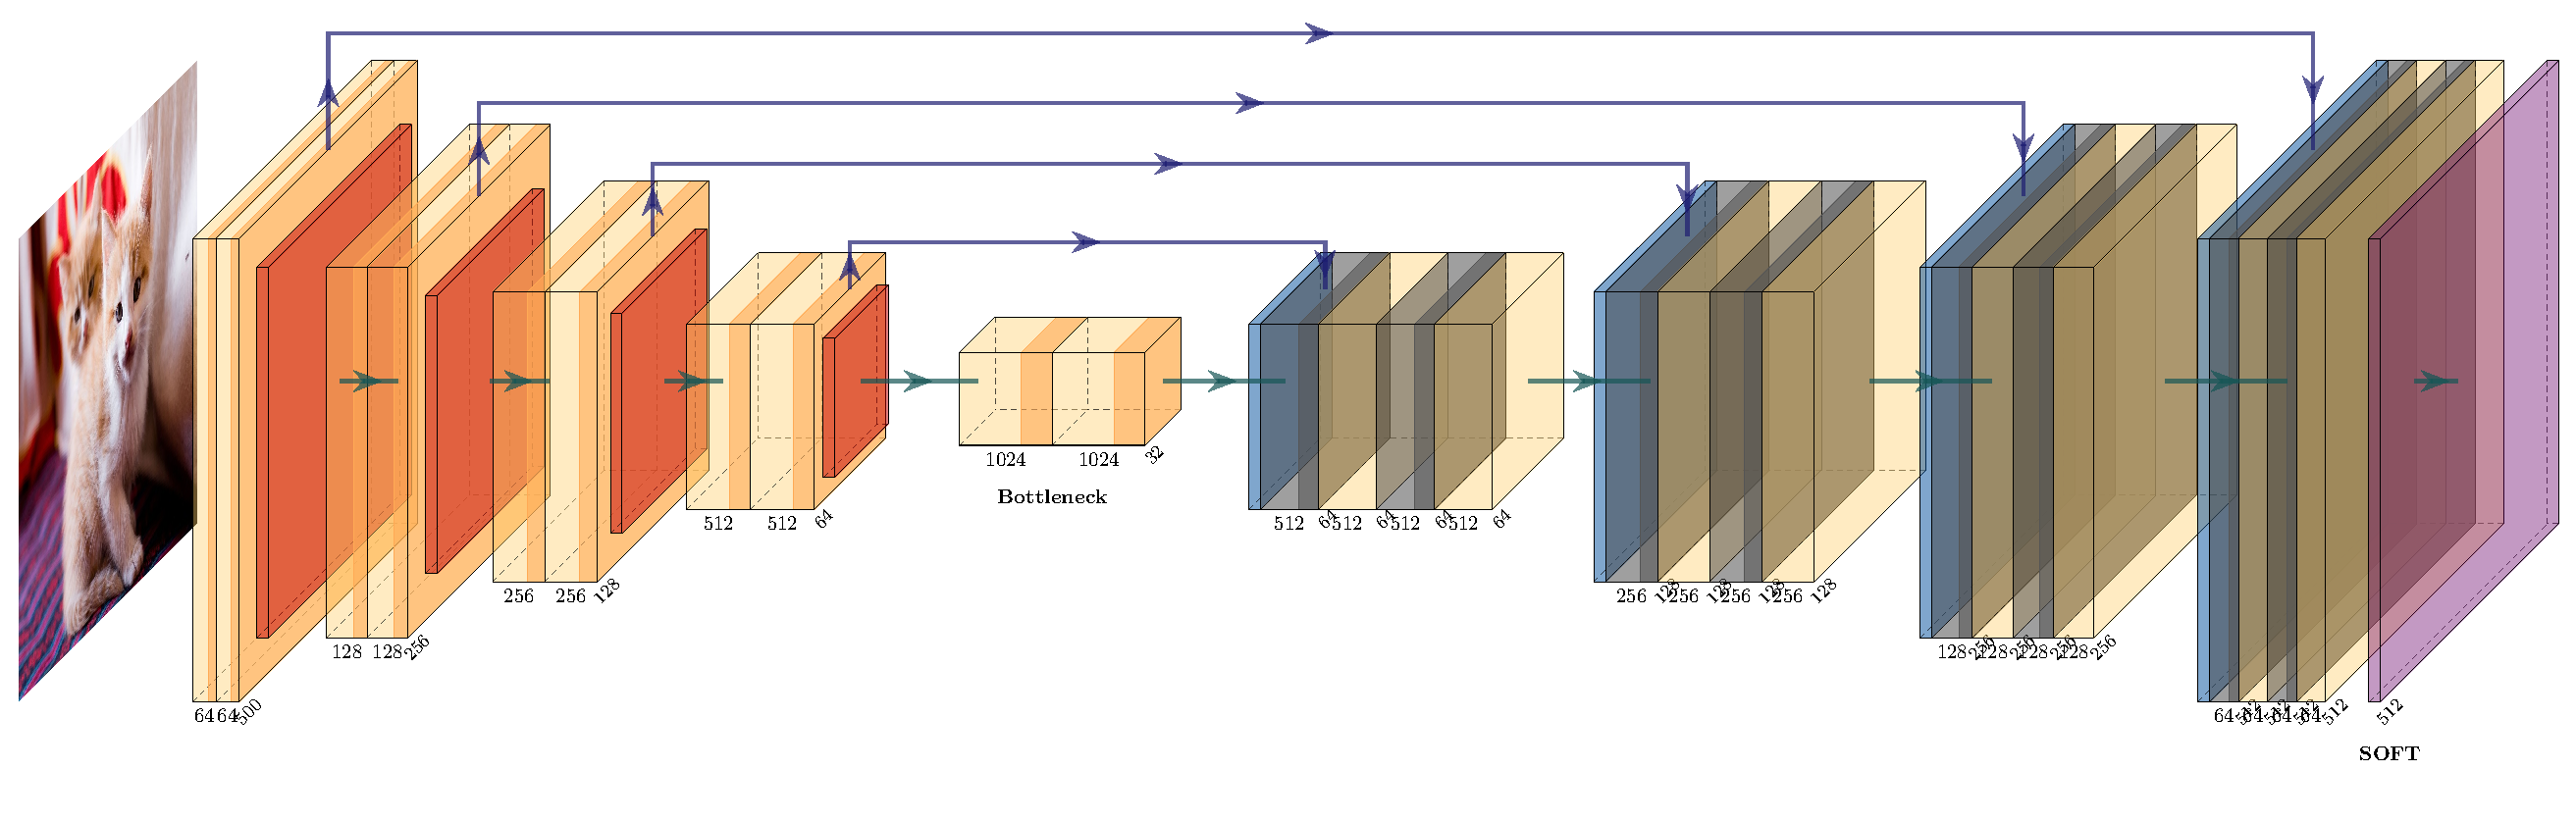
\includegraphics[width=0.45\textwidth]{unet.pdf}}
    \caption{U-Net architecture (same as exp7/exp8).}
    \label{fig:unet}
\end{figure}

The U-Net structure consists of:

(1) \textbf{Encoder}: 4 down-sampling blocks (Conv-BN-ReLU $\times$ 2 + MaxPool).

(2) \textbf{Bottleneck}: 1024 channels, two convolution blocks.

(3) \textbf{Decoder}: 4 up-sampling blocks with transposed convolutions and skip connections.

(4) \textbf{Output layer}: $1 \times 1$ convolution for residual noise estimation.

During inference, the full noisy image is directly passed through the trained U-Net to produce the denoised output without any sub-sampling.

\section{Experiment}

\subsection{Dataset and experimental setup}

Consistent with exp7 and exp8, we use the DIV2K dataset. For each image patch, we generate a single additive white Gaussian noise (AWGN) realization. The training set comprises 200 high-resolution images.

(1) \textbf{Optimizer}: Adam with initial learning rate $1 \times 10^{-3}$.

(2) \textbf{Scheduler}: Cosine Annealing schedule.

(3) \textbf{Loss function}: MSE (Reconstruction Loss) + Regularization Loss ($\gamma = 2.0$).

(4) \textbf{Sub-sampling}: Random row or column spatial down-sampling.

(5) \textbf{Epochs}: 50, consistent with exp7 and exp8.

\subsection{Experimental content}

\subsubsection{Quantitative results}

After training, the Neighbor2Neighbor model is evaluated on the validation set. Table~\ref{tab:gray} shows the generalization results across multiple noise levels for the grayscale model.

\begin{table}[htbp]
\caption{Neighbor2Neighbor grayscale model evaluation}
\begin{center}
\begin{tabular}{cccc}
\toprule
\textbf{$\sigma$} & \textbf{Method} & \textbf{PSNR (dB)} & \textbf{SSIM} \\
\midrule
15 & Neighbor2Neighbor & 29.46 & 0.7514 \\
25 & Neighbor2Neighbor & 28.63 & 0.7406 \\
35 & Neighbor2Neighbor & 24.06 & 0.5058 \\
50 & Neighbor2Neighbor & 18.59 & 0.2737 \\
\bottomrule
\end{tabular}
\label{tab:gray}
\end{center}
\end{table}

\subsubsection{Comparison with previous methods}

Table~\ref{tab:comparison} compares the N2N model with all baseline methods from previous experiments at $\sigma=25$ on grayscale images.

\begin{table}[htbp]
\caption{Comparison with all methods on grayscale images ($\sigma=25$)}
\begin{center}
\resizebox{\columnwidth}{!}{%
\begin{tabular}{lccc}
\toprule
\textbf{Method} & \textbf{Data requirement} & \textbf{PSNR (dB)} & \textbf{SSIM} \\
\midrule
ADMM & None (optimization) & 27.75 & 0.6438 \\
BM3D & None (traditional) & 29.70 & 0.7963 \\
DnCNN & Noisy + Clean & 29.99 & 0.8148 \\
Supervised U-Net (exp7) & Noisy + Clean & 29.60 & 0.7523 \\
Noise2Noise (exp8) & Noisy Pair & 28.40 & 0.7302 \\
\midrule
\textbf{N2N (exp9)} & \textbf{Single Noisy} & \textbf{28.63} & \textbf{0.7406} \\
\bottomrule
\end{tabular}}
\label{tab:comparison}
\end{center}
\end{table}

\subsubsection{Visual comparison}

Visual results for grayscale denoising at $\sigma=25$ are presented in Fig.~\ref{fig:gray}. The denoised output demonstrates effective noise removal while preserving structural details such as edges and textures.

\begin{figure}[htbp]
    \centerline{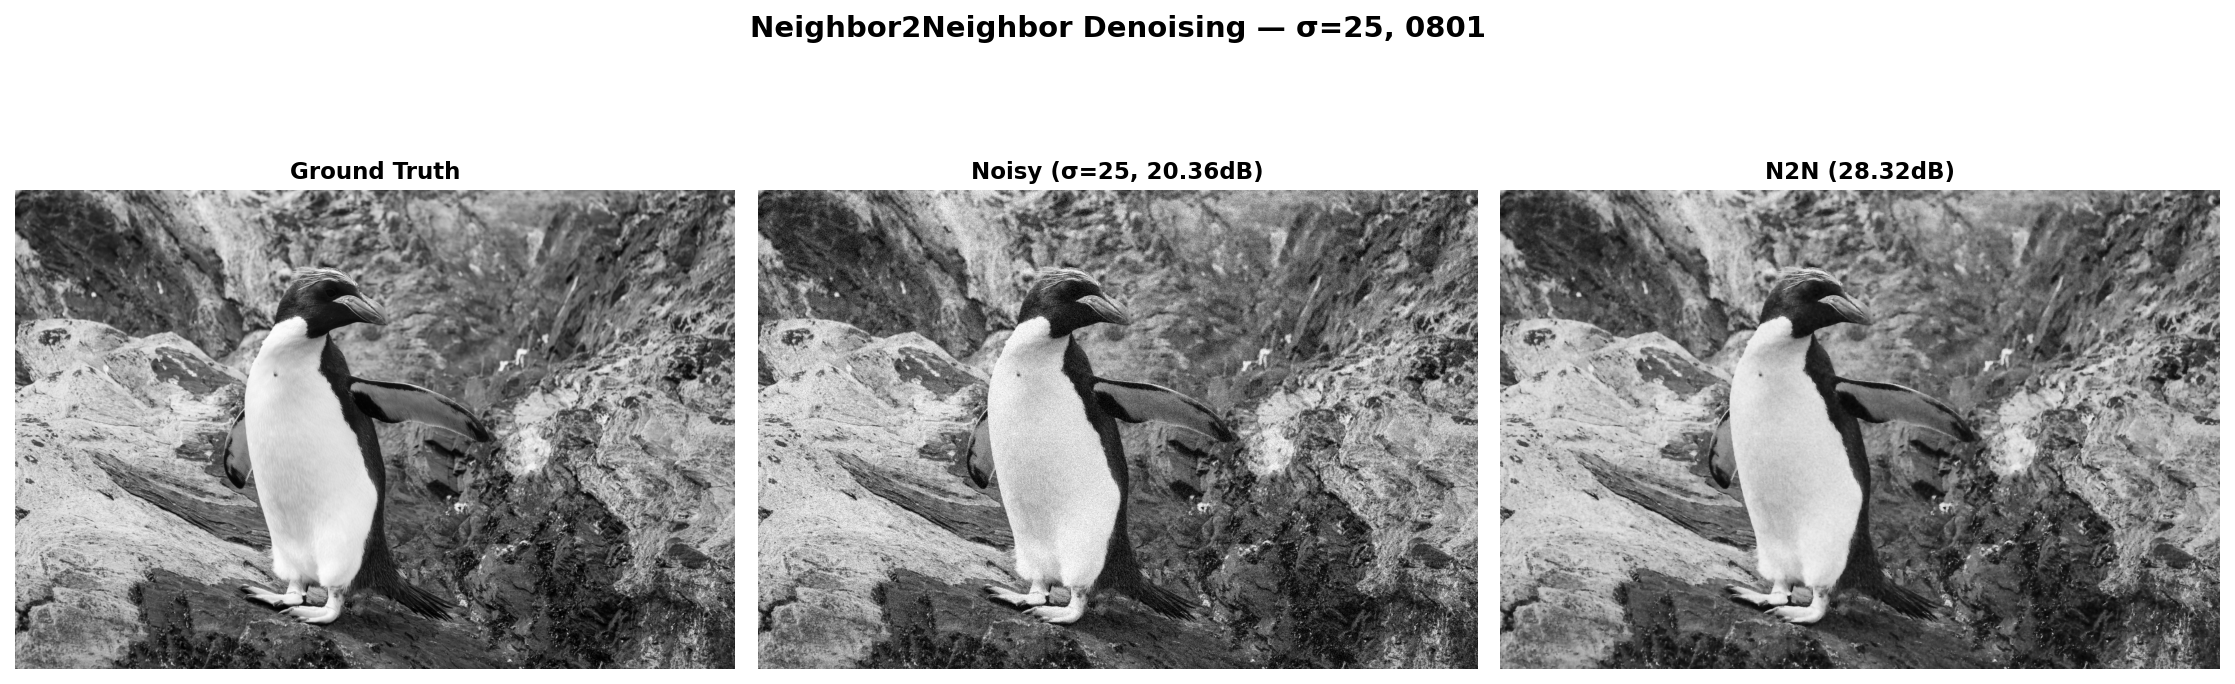
\includegraphics[width=0.45\textwidth]{visual_gray_sigma25_0801.png}}
    \caption{Neighbor2Neighbor grayscale denoising ($\sigma=25$).}
    \label{fig:gray}
\end{figure}

\subsection{Running time and efficiency}

During inference, Neighbor2Neighbor uses the same U-Net forward pass as exp7 and exp8. The computation involved in sub-sampling and regularization occurs strictly during training, leading to identical test-time efficiency as standard supervised pipelines.

\section{Conclusion and discussion}

In this study, we implemented and evaluated a Neighbor2Neighbor self-supervised denoiser, completing the progression from supervised learning (exp7) through paired self-supervision (exp8) to single-image self-supervision (exp9). The key findings are:

(1) \textbf{Data efficiency}: N2N successfully trains with only single noisy images via sub-sampling. It stands out in practical scenarios where collecting paired dataset is unfeasible.

(2) \textbf{Performance trade-off}: The reduced data requirement leads to a minor performance trade-off compared to paired or explicitly supervised baselines, as the network relies on sub-sampled estimates and spatial correlations.

(3) \textbf{Regularization value}: Incorporating the regularization loss handles the gap between pseudo-pairs effectively, addressing the noise independence issue and matching the true discrepancy.

Future work could explore optimizing the sub-sampling process dynamically or learning the regularization boundary with advanced heuristics.

\begin{thebibliography}{00}
\bibitem{b1} T. Huang, S. Li, X. Jia, H. Lu, and J. Liu, ``Neighbor2Neighbor: Self-supervised denoising from single noisy images,'' in Proc. CVPR, 2021, pp. 14781--14790.
\bibitem{b2} A. Krull, T. Buchholz, and F. Jug, ``Noise2Void -- Learning denoising from single noisy images,'' in Proc. CVPR, 2019, pp. 2129--2137.
\bibitem{b3} J. Batson and L. Royer, ``Noise2Self: Blind denoising by self-supervision,'' in Proc. ICML, 2019, pp. 524--533.
\end{thebibliography}

\end{document}
